\def\year{2022}\relax
%File: formatting-instructions-latex-2022.tex
%release 2022.1
\documentclass[letterpaper]{article} % DO NOT CHANGE THIS
\usepackage{aaai22}  % DO NOT CHANGE THIS
\usepackage{times}  % DO NOT CHANGE THIS
\usepackage{helvet}  % DO NOT CHANGE THIS
\usepackage{courier}  % DO NOT CHANGE THIS
\usepackage[hyphens]{url}  % DO NOT CHANGE THIS
\usepackage{graphicx} % DO NOT CHANGE THIS
\urlstyle{rm} % DO NOT CHANGE THIS
\def\UrlFont{\rm}  % DO NOT CHANGE THIS
\usepackage{natbib}  % DO NOT CHANGE THIS AND DO NOT ADD ANY OPTIONS TO IT
\usepackage{caption} % DO NOT CHANGE THIS AND DO NOT ADD ANY OPTIONS TO IT
\DeclareCaptionStyle{ruled}{labelfont=normalfont,labelsep=colon,strut=off} % DO NOT CHANGE THIS
\frenchspacing  % DO NOT CHANGE THIS
\setlength{\pdfpagewidth}{8.5in}  % DO NOT CHANGE THIS
\setlength{\pdfpageheight}{11in}  % DO NOT CHANGE THIS
%
% These are recommended to typeset algorithms but not required. See the subsubsection on algorithms. Remove them if you don't have algorithms in your paper.
% \usepackage{algorithm}
% \usepackage{algorithmic}

%
% These are are recommended to typeset listings but not required. See the subsubsection on listing. Remove this block if you don't have listings in your paper.
% \usepackage{newfloat}
\usepackage{listings}
\lstset{%
	basicstyle={\footnotesize\ttfamily},% footnotesize acceptable for monospace
	numbers=left,numberstyle=\footnotesize,xleftmargin=2em,% show line numbers, remove this entire line if you don't want the numbers.
	aboveskip=0pt,belowskip=0pt,%
	showstringspaces=false,tabsize=2,breaklines=true}

%
\nocopyright
%
% PDF Info Is REQUIRED.
% For /Title, write your title in Mixed Case.
% Don't use accents or commands. Retain the parentheses.
% For /Author, add all authors within the parentheses,
% separated by commas. No accents, special characters
% or commands are allowed.
% Keep the /TemplateVersion tag as is
\pdfinfo{
/Title (AAAI Press Formatting Instructions for Authors Using LaTeX -- A Guide)
/Author (AAAI Press Staff, Pater Patel Schneider, Sunil Issar, J. Scott Penberthy, George Ferguson, Hans Guesgen, Francisco Cruz, Marc Pujol-Gonzalez)
/TemplateVersion (2022.1)
}

\usepackage{graphicx}
\usepackage[export]{adjustbox}
\usepackage{amssymb}
\usepackage{amsmath}
\usepackage{algorithm}
\usepackage{algorithmic}
\usepackage{booktabs}
\usepackage{subfigure}

% DISALLOWED PACKAGES
% \usepackage{authblk} -- This package is specifically forbidden
% \usepackage{balance} -- This package is specifically forbidden
% \usepackage{color (if used in text)
% \usepackage{CJK} -- This package is specifically forbidden
% \usepackage{float} -- This package is specifically forbidden
% \usepackage{flushend} -- This package is specifically forbidden
% \usepackage{fontenc} -- This package is specifically forbidden
% \usepackage{fullpage} -- This package is specifically forbidden
% \usepackage{geometry} -- This package is specifically forbidden
% \usepackage{grffile} -- This package is specifically forbidden
% \usepackage{hyperref} -- This package is specifically forbidden
% \usepackage{navigator} -- This package is specifically forbidden
% (or any other package that embeds links such as navigator or hyperref)
% \indentfirst} -- This package is specifically forbidden
% \layout} -- This package is specifically forbidden
% \multicol} -- This package is specifically forbidden
% \nameref} -- This package is specifically forbidden
% \usepackage{savetrees} -- This package is specifically forbidden
% \usepackage{setspace} -- This package is specifically forbidden
% \usepackage{stfloats} -- This package is specifically forbidden
% \usepackage{tabu} -- This package is specifically forbidden
% \usepackage{titlesec} -- This package is specifically forbidden
% \usepackage{tocbibind} -- This package is specifically forbidden
% \usepackage{ulem} -- This package is specifically forbidden
% \usepackage{wrapfig} -- This package is specifically forbidden
% DISALLOWED COMMANDS
% \nocopyright -- Your paper will not be published if you use this command
% \addtolength -- This command may not be used
% \balance -- This command may not be used
% \baselinestretch -- Your paper will not be published if you use this command
% \clearpage -- No page breaks of any kind may be used for the final version of your paper
% \columnsep -- This command may not be used
% \newpage -- No page breaks of any kind may be used for the final version of your paper
% \pagebreak -- No page breaks of any kind may be used for the final version of your paperr
% \pagestyle -- This command may not be used
% \tiny -- This is not an acceptable font size.
% \vspace{- -- No negative value may be used in proximity of a caption, figure, table, section, subsection, subsubsection, or reference
% \vskip{- -- No negative value may be used to alter spacing above or below a caption, figure, table, section, subsection, subsubsection, or reference

\setcounter{secnumdepth}{0} %May be changed to 1 or 2 if section numbers are desired.

% The file aaai22.sty is the style file for AAAI Press
% proceedings, working notes, and technical reports.
%

% Title

% Your title must be in mixed case, not sentence case.
% That means all verbs (including short verbs like be, is, using,and go),
% nouns, adverbs, adjectives should be capitalized, including both words in hyphenated terms, while
% articles, conjunctions, and prepositions are lower case unless they
% directly follow a colon or long dash
\title{Traffic Signal Control based on Reinforcement Learning}
\author{
    %Authors
    % All authors must be in the same font size and format.
    Chixuan Zhang,
    Hairui Yin,
    Yida Qiu,
    Yukun Qi,
}
\affiliations{
    %Afiliations
    % If you have multiple authors and multiple affiliations
    % use superscripts in text and roman font to identify them.
    % For example,

    % Sunil Issar, \textsuperscript{\rm 2}
    % J. Scott Penberthy, \textsuperscript{\rm 3}
    % George Ferguson,\textsuperscript{\rm 4}
    % Hans Guesgen, \textsuperscript{\rm 5}.
    % Note that the comma should be placed BEFORE the superscript for optimum readability
	ShanghaiTech University\\
	393 Middle Huaxia Road, Pudong, Shanghai\\
    % email address must be in roman text type, not monospace or sans serif
    zhangchx@shanghaitech.edu.cn,
    yinhr@shanghaitech.edu.cn\\
    qiuyd@shanghaitech.edu.cn,
    qiyk@shanghaitech.edu.cn
%
% See more examples next
}

%Example, Single Author, ->> remove \iffalse,\fi and place them surrounding AAAI title to use it
\iffalse
\title{My Publication Title --- Single Author}
\author {
    Author Name
}
\affiliations{
    Affiliation\\
    Affiliation Line 2\\
    name@example.com
}
\fi

\iffalse
%Example, Multiple Authors, ->> remove \iffalse,\fi and place them surrounding AAAI title to use it
\title{My Publication Title --- Multiple Authors}
\author {
    % Authors
    First Author Name,\textsuperscript{\rm 1}
    Second Author Name, \textsuperscript{\rm 2}
    Third Author Name \textsuperscript{\rm 1}
}
\affiliations {
    % Affiliations
    \textsuperscript{\rm 1} Affiliation 1\\
    \textsuperscript{\rm 2} Affiliation 2\\
    firstAuthor@affiliation1.com, secondAuthor@affilation2.com, thirdAuthor@affiliation1.com
}
\fi


% REMOVE THIS: bibentry
% This is only needed to show inline citations in the guidelines document. You should not need it and can safely delete it.
\usepackage{bibentry}
% END REMOVE bibentry

\begin{document}

\maketitle

\begin{abstract}
We realize and compare several traffic controlling methods based on Random, Greedy Algorithm, naive Q-learning, Periodic Cycle and deep Q-network. The simulation environment of our project is built on Simulation of Urban Mobility (SUMO) where Road traffic can be visualized and vehicles and road information can be easily extracted. In our methods, the evaluation criteria are set according to the total waiting time of all cars in the simulation and the length of different lanes. Greedy Algorithm modulates traffic light according to lanes length. Naive Q-learning updates q value according to state and action. Periodic Cycle is the same as our real world where the period is determined by experience. In our code, the period is selected after tests. Deep Q-network (DQN) is the combination of Reinforcement Learning (RL) and Deep Learning (DL).
The achieved results show that DQN algorithm can produce intelligent behavior.
\end{abstract}

\section{1\ \ \ Introduction}

\hspace*{1em}Traffic congestion is a complex and pervasive issue facing highly urbanized countries around the world. By addressing traffic congestion, it is possible to reduce fuel consumption, decrease delays, and improve logistics transportation. Traditional traffic light control policies often rely on historical data and are adjusted according to specific times of day, but these methods are often ineffective and struggle to reach optimal performance. As a result, drivers may find themselves waiting at red traffic lights even when no other vehicles are present. However, the development of vehicular communication technologies offers an opportunity to gather more detailed information about vehicles, which can be used in conjunction with computational methods to improve traffic flow through more efficient traffic light control policies. In the future, the integration of autonomous driving technologies may further enhance the performance of these policies.

Markov Decision Processes (MDPs) and Traditional Reinforcement Learning (RL) frameworks are popular approaches for optimizing traffic light control policies as they can achieve optimal performance through techniques such as policy iteration, value iteration, and linear programming. However, both MDPs and RL frameworks suffer from issues related to high dimensionality, resulting in large state spaces and slow convergence in real-world problems. The optimal performance of these approaches is therefore difficult to attain due to the significant computational power required. To address these challenges, we propose the use of Deep Q-Networks to optimize a realistic traffic light control problem and achieve a local optimal solution. We explored the potential of Deep Q-Networks in this application by comparing them to other methods (including Random, Period Control, Greedy Algorithm, $\epsilon$-Greedy, Naive Q-learning) and identifying other potential ways to improve traffic light control strategies.

\subsection{1.1 External Libraries}
\paragraph{SUMO} SUMO, Simulation of Urban Mobility, is an open source, micro, multimodal traffic simulation software developed in 2000. It is purely microscopic and can be controlled individually for each vehicle, so it is very suitable for the development of traffic control models. SUMO can give each vehicle a unique identifier, departure time, and route, as well as customize its lane, speed, or location.

\paragraph{PyTorch} PyTorch is one of the most popular deep learning frameworks. It is simple, efficient and fast. To keep our project relevant to the course, PyTorch was used only to help us implement a Multi-Layer Perceptron (MLP) and assist in training the model.

% \subsection{Contribution}

\section{2\ \ \ Related Work}
\hspace*{1em}There has been growing interest in using reinforcement learning (RL) to optimize traffic signal control methods. However, many existing machine learning approaches do not adequately compare with classical transportation methods, which have been largely ignored. Hua Wei (2020) conducted a survey that takes a comprehensive view of both machine learning and transportation engineering in order to facilitate interdisciplinary research and bridge this gap.

Several classical transportation methods have been identified for comparison as baselines for RL-based methods, including Webster, GreenWave, Maxband, Actuated, SOTL, Max-pressure, and SCATS. These methods use various inputs, such as traffic volume, phase sequence, lane length, speed limit, and queue length, to generate cycle-based signal plans for individual intersections and offsets between adjacent traffic signals. Webster generates a signal plan for a single intersection using traffic volume and phase sequence, while GreenWave and Maxband determine offsets for a cycle-based signal plan using traffic volume, lane length, speed limit, and a cycle-based signal plan at individual intersections. Actuated and SOTL use traffic volume, phase sequence, and a phase change rule to determine the transition to the next phase. Max-pressure control aims to minimize the "pressure" of phases at an intersection in order to balance queue length between neighboring intersections and reduce the risk of over-saturation. SCATS uses pre-defined signal plans and performance measurements to adjust signal plans for all intersections based on traffic volume.

Several artificial intelligence techniques have been proposed for use in traffic signal control, including fuzzy logic algorithms, swarm intelligence, and reinforcement learning. Examples of these approaches include the use of fuzzy logic algorithms [Gokulan and Srinivasan 2010], swarm intelligence [Teodorović 2008], and reinforcement learning [ElTantawy 2012; Kuyer 2008; Mannion 2016; Wiering 2000].

\section{3\ \ \ Problem Statement}
\hspace*{1em}We model the road intersections and formulate our optimization problem. For the sake of transparency, we consider an admittedly stylized simulation that only aims to capture the most essential features that govern the dynamics of contending traffic flows at road intersections. We throughout adopt a discrete time formulation to simplify the description according to our iteration and allow comparision of all methods based on the same total cars amount and lane-based speed control.
\subsection{3.1 Crossroad}
\hspace*{1em}Our simulation starts with a single-intersection scenario to facilitate the validation of RL algorithms by comparing with all used approaches. We consider the simplest meaningful setup with directional crossroads traffic flows as schematically depicted in the picture.
\begin{figure}[h]
	\centering
	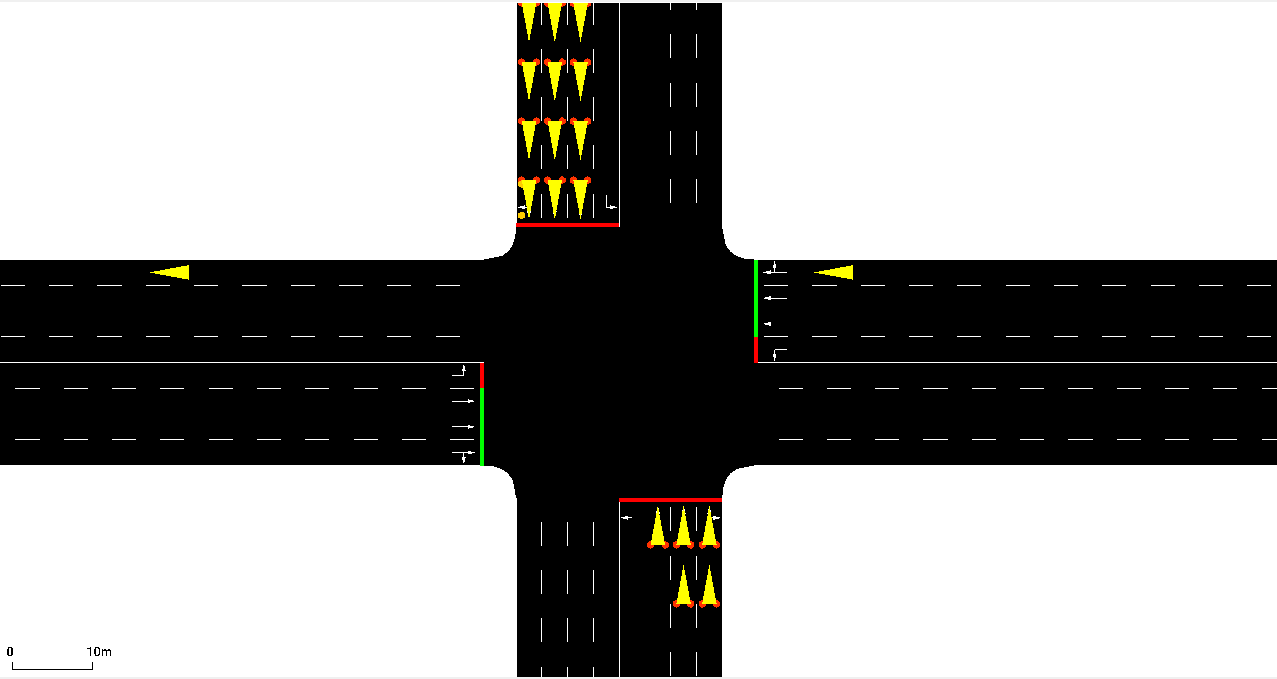
\includegraphics[width=0.9\linewidth, frame]{crossroad}
	\caption{Crossroad}
	\label{fig:crossroad}
\end{figure}
\newline
\hspace*{1em}This is a traffic intersection with a total of four roads at the junction, of which each road has eight lanes, four heading towards the junction and four heading outwards. Vehicles in the outward lane can pass directly, while vehicles in the inward lane need to follow the traffic signal. There are four kinds of inward lanes with different legal actions:
\begin{itemize}
	\item 0: turn right or go ahead
	\item 1,2: only go ahead
	\item 3: only turn left
\end{itemize}
\subsection{3.2 Traffic Light Control}
\hspace*{1em}In reality, most traffic lights change in the same direction, meaning that the opposite road of an intersection will change green at a time. So in our simulation, we follow the same guidelines and have four traffic light operations:
\begin{itemize}
	\item Lights in straight lanes of left and right roads are green, the rest are all red
	\item Lights in leftturn lanes of left and right roads are green, the rest are all red
	\item Lights in straight lanes of up and down roads are green, the rest are all red
	\item Lights in leftturn lanes of up and down roads are green, the rest are all red
\end{itemize}
\hspace*{1em}Note that we only consider the red and green light conditions, not the yellow light condition. Traffic lights also change in an instant.
\subsection{3.3 Evaluation criteria}
\hspace*{1em}During our simulation iteration, we can obtain information of all vehicles and roads. Considering our real life, traffic congestion happens when queue is long and every vehicle has to wait for a long time. And the car at the front of congestion may have shorter waiting time while waiting time of cars at the end is larger. As a result, in our code, we consider the total waiting time of every vehicle and the variance of cars' waiting time as evaluation criteria.
$$
T_S = \sum^N_{i=1}T(i)
$$
$$
\sigma^2 = \frac{\sum^N_{i=1}(T(i)-\bar{T})}{N}
$$
where $T_S$ is the total waiting time, $T(i)$ is the waiting time of vehicle $i$, $\sigma$ is the variance, $N$ is the total amount of vehicles and $\bar{T}$ is the average waiting time.
\subsection{3.4 Optimization Goal}
\hspace*{1em}We assume that after all iterations, the total waiting time $T_S$ and the waiting time variance$\sigma$ are calculated. The goal is to a dynamic control policy which selects actions over time so as to minimize $T_S$ and $\sigma$.

\section{4\ \ \ Method}

\subsection{4.1 Q-Learning}
\hspace*{1em}Q-leaning is a model-free reinforcement learning technique proposed by Watkins el al. in 1989. It has been proved that Q-learning will eventually find an optimal strategy for any finite Markov Decision Processes (MDPs).
\vspace*{0.1cm}

In Q-learning, actions are selected based on their expected reward $r_t$. The goal is to choose the action that will result in the maximum reward for a given state. The iterative process of value function is the core of Q-learning.
\begin{small}
	$$Q(s_t,a_t)\leftarrow Q(s_t,a_t)+\alpha\cdot\left[r_t+\gamma\max_\pi Q(s_{t+1},a_t)-Q(s_t,a_t)\right]$$
\end{small}\noindent

Where $\alpha$ is the learning rate and $\gamma$ is the discount factor. $\alpha$ helps to avoid getting stuck in a locally optimal solution. Higher alpha values result in faster changes to Q-values. And $\gamma$ determines the importance of future rewards by multiplying the estimated optimal future value in the Q-learning equation. In the Q-learning equation, the new Q-value for a state is calculated by adding the selected action's Q-value to the old Q-value.

However, when facing state space in high dimesion, it's easy for Q-learning to meet problem of Dimensional curse and memory difficulties. Unfortunately, most data in the real world is high dimensional. For example, in our task, we only consider the number of cars on each road (16 roads in total), and suppose there are at most 15 cars on one road at a time, the state space will be $15^{16}\approx 6.57\times 10 ^{18}$. At least right now, it's impossible for us to solve this problem. And the real problem is more complex and even has continuous features. Hence, we need to consider some approximate methods.

\subsection{4.2 Q-learning with {\huge $\epsilon$}-Greedy}

\hspace*{1em}The {\large $\epsilon$}-greedy action selection method combines exploitation, in which the agent makes use of prior knowledge to maximize reward, with exploration, in which the agent searches for new options. Most of the time, the $\epsilon$-greedy approach will select the action with the highest estimated reward. However, with a small probability epsilon, the agent will choose to explore by selecting an action randomly, regardless of its estimated reward. This allows the agent to try new things and potentially discover better options. Through infinite trials, the $\epsilon$-greedy action selection policy is able to discover the optimal actions. With this idea, we can update the value iteration equation as below:
\begin{align*}
	&Q(s_t,a_t)\leftarrow Q(s_t,a_t)+\alpha\cdot\left[r_t+\gamma\cdot\mathbb{Q}-Q(s_t,a_t)\right]\\
	&\mathbb{Q} = \begin{cases}
		\max_\pi Q(s_{t+1},a_t),\ &\text{with probabilty}\ 1-\epsilon\\
		Q(s_{t+1},a_{\text{random}}),\ &\text{with probabilty}\ \epsilon
	\end{cases}
\end{align*}

\subsection{4.3 Deep Q-Network}

\hspace*{1em}To deal with the weakness of Q-learning about high dimensional data. We can use a neural network to approximate the value function. $\hat{Q}_\theta(s,a)\approx Q(s,a)$ The value iterative process can be denoted as: 
\begin{small}
	$$\hat{Q}(s_t,a_t)\leftarrow \hat{Q}(s_t,a_t)+\alpha\cdot\left[r_t+\gamma\max_\pi \tilde{Q}(s_{t+1},a_t)-\hat{Q}(s_t,a_t)\right]$$
\end{small}
\hspace*{1em}Where $\hat{Q}(s_t,a_t)$ is the main neural network in training, and $\tilde{Q}(s_{t+1},a_t)$ is the targetNet (more contents below). A good model should be able to achieve the most likely output action is the decision that makes Q-value be best.

\paragraph{Model Snapshot} In order to avoid the problem that model doesn't convergence, we do not use the real-time update model, but use a snapshot of model. In other words, every K steps, the model is stored and fixed as a snapshot for computing ideal Q, which is also called target network.

\paragraph{Experience Replay} MultiLayer Perceptron (Deep Neural Network) is a supervised learning model, which asks the data should be independent and identically distributed. Experience Replay breaks down the correlation by the store-sampling method. Save the data from the environment agent and then sample from the data.

\begin{figure}[h]
	\centering
	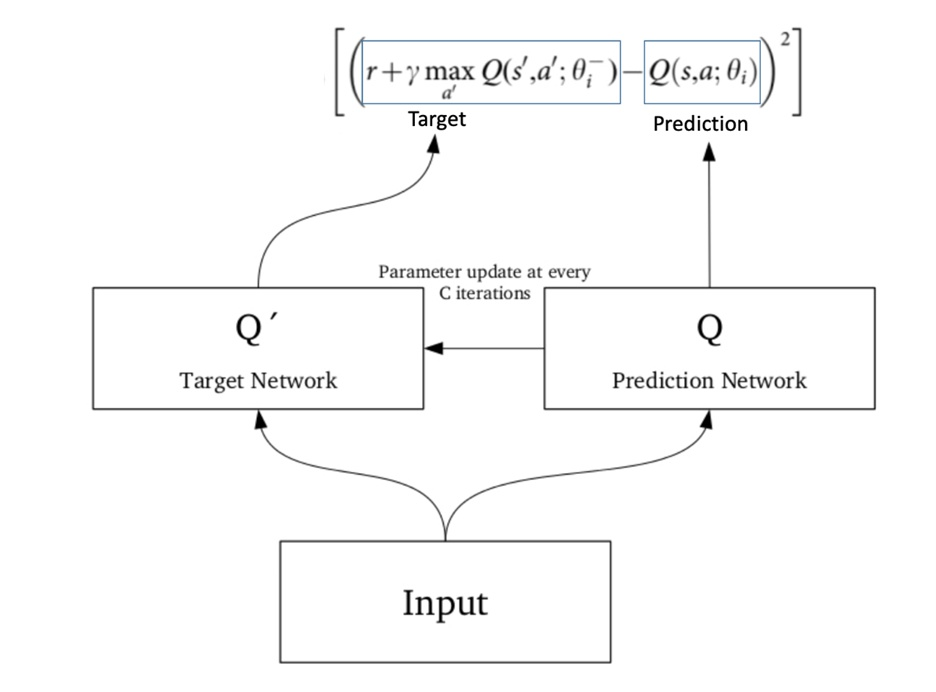
\includegraphics[width=0.8\linewidth, frame]{DQN}
	\caption{Deep Q-Learning Framework}
	\label{fig:dqn}
\end{figure}

\subsection{4.4 DQN Algorithm Design}
\hspace*{1em}We provide a detailed pseudo-code and detailed parameters setting of the DQN algorithms for the scenarios of a single intersection as described in the previous section.

To ensure relevance to the course content, we will use a simple Multi-Layer Perceptron as the neural network to fit the $Q(s_t,a_t)$. The MLP has four hidden layers of 400 nodes, and the input is a 16-length tensor, which is the number of cars on the 16 roads. And the output is a 4-length tensor to give the score of 4 actions.
$$Loss(\theta) = \mathbb{E}\left[\left(r+\gamma\max_{a'} \tilde{Q}(s',a')-\hat{Q}(s,a)\right)^2\right]$$

The loss function is as above, where $r$ is the reward in the current step, $r$ is calculated by the difference between the total waiting time of the current time step and the next. $\gamma$ is the discount factor for acceleration of convergence. And $\tilde{Q}(s',a')$ is the target model, which is a copy for the main model $\hat{Q}(s,a)$ for each 1 step.

\begin{algorithm}[h]
	\caption{Deep Q-Network Algorithm for SUMO} % 名称
	\label{alg::conjugateGradient}
	\begin{algorithmic}[1]
		\REQUIRE
		$Q_\theta$: the model need to be learned;
		\ENSURE
		Q-value interative equation is satisfied
		\STATE initial target model $\mathbb{Q}=Q_\theta$;
		\FOR{epoch $<$ MAXEPOCH}
		\WHILE{SUMO is runing}
		\STATE $\epsilon=1-\text{epoch}/\text{MAXEPOCH}$
		\STATE $a_t$ = epsilonGreedy($\epsilon$)
		\STATE $s_t$ = getfeatures()
		\STATE $q_t$ = $\mathbb{Q}(s_t, a_t)$
		\ENDWHILE
		\FOR{i $<$ MAXITERATION}
		\FOR{batch in Experience Replay}
		\STATE LOSS$\left(Q_\theta(s_t), a_t, q_{t+1}\right)$
		\STATE OPTIMIZER($Q_\theta$, learning\_rate)
		\ENDFOR
		\ENDFOR
		\STATE Every 1 Epoch, Update $\mathbb{Q}=Q_\theta$.
		\STATE SAVE CheckPoints $Q_\theta$
		\ENDFOR
	\end{algorithmic}
\end{algorithm}
\newpage

\section{5\ \ \ Experiment}
\hspace*{1em}In this section, we quantitatively evaluate traditional method based on empirical periodic setting. And four different periods are used. Following existing period work, we test all proposed methods as well as the competitive baselines. We first present the general experiment setups, and then describe task-specific evaluation protocols and discuss the results in each section.
\subsection{5.1 Experiment Setup}
\paragraph{Baselines} The traditional method in traffic light control field is Periodic Cycle control. Four different Periodic Cycle parameters are set. The parameters with the best simulation performance is chosen as the baseline. 
\subsection{5.2 Experiment Detail}
\paragraph{Evaluation Criteria} As mentioned in $3.3$, the total waiting time $T_S$ of all vehicles and the variance of time $\sigma$ between each car are recorded and set as the Evaluation Criteria. $T_S$ measures the overall performance of the method. And $\sigma$ measures fairness between vehicles, a higher $\sigma$ means there exists some vehicles having to wait for a long time.
\paragraph{Multiple experiments} For every method, multiple tests with different random seed are operated in order to reduce the impact of randomness. The result taken into consideration is the average result of each method.
\paragraph{DQN HyperParameters} The complete Deep Q-Network Algorithm and loss function is in section4.4. Here are some other concrete hyperparameters. MAXEPOCH is set as 100. MAXITERATION is set as 800. SUMO will be run for 5400 ticks in one epoch. And we choose Adam algorithm (which is the only content in our project that is not related to the course) to be the optimizer with learning rate $1e-3$. One epoch needs about 40s on a 6900xt gpu.

\subsection{5.3 Experiment Result}
\begin{table}[htbp]
	\centering
	\renewcommand\arraystretch{1.5}
	\caption{Results on different method}
	\setlength{\tabcolsep}{6mm}{
		\begin{tabular}{ c | c | c }
			\toprule
			Method Name & $T_S$ & $\sigma$\\
			\hline
			Deep Q-Network & 15908.0 & 461.22\\
			
			Greedy & 16850.0 & 834.02\\
			
			Period Cycle & 47942.0 & 1681.86\\
			
			Random & 62800.0 & 868.04\\
			
			SUMO buildin & 75467.0 & 839.59\\
			\bottomrule
	\end{tabular}}
\end{table}
The result is summarized in Table 1 and has been sorted according to their performance. In the result, under the same vehicle circumstance, Deep Q-Network performs best, both in total time and variance. Greedy has a similar total time, but a much larger variance. Period Cycle, as a baseline, has a relatively average performance, of which total time is approximately three time larger than these two methods above but better than completely python determined random and SUMO buildin random. And the periodic method has the largeset variance.

\paragraph{Waiting Time Analysis} During iteration, the accumulative waiting time $T_S$ is in Figure 3. A figure with only performance of DQN and Greedy is intended to show the difference between them more clearly.
\begin{figure}[h]
	\centering
	\subfigure[All methods]{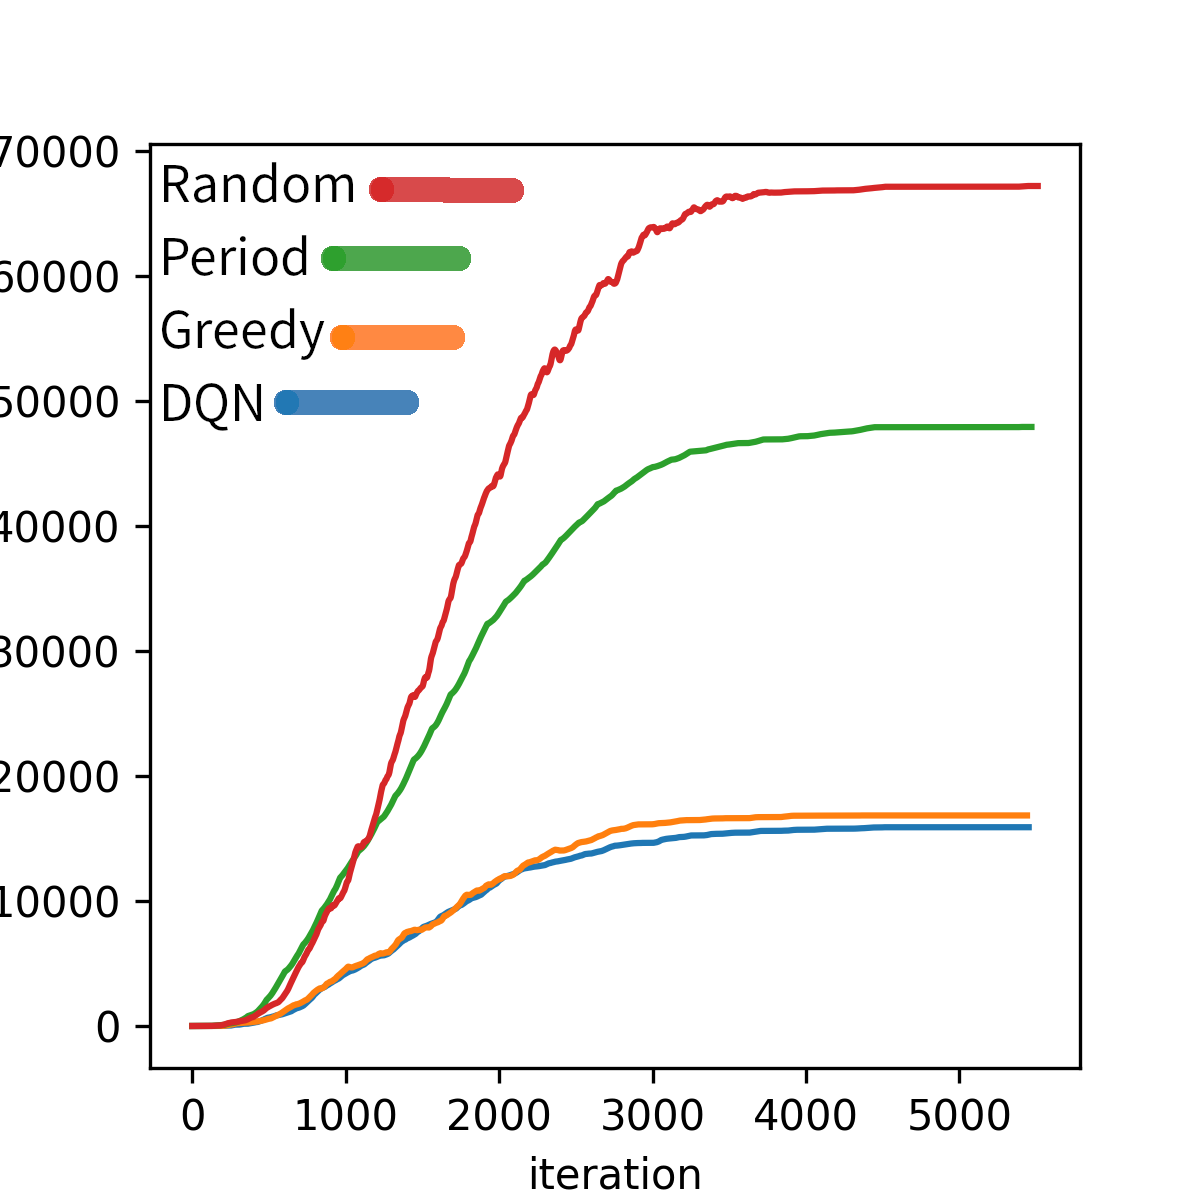
\includegraphics[width=4cm]{waiting_time1.png}} %[图片大小]{图片路径}
	\subfigure[DQN and Greedy]{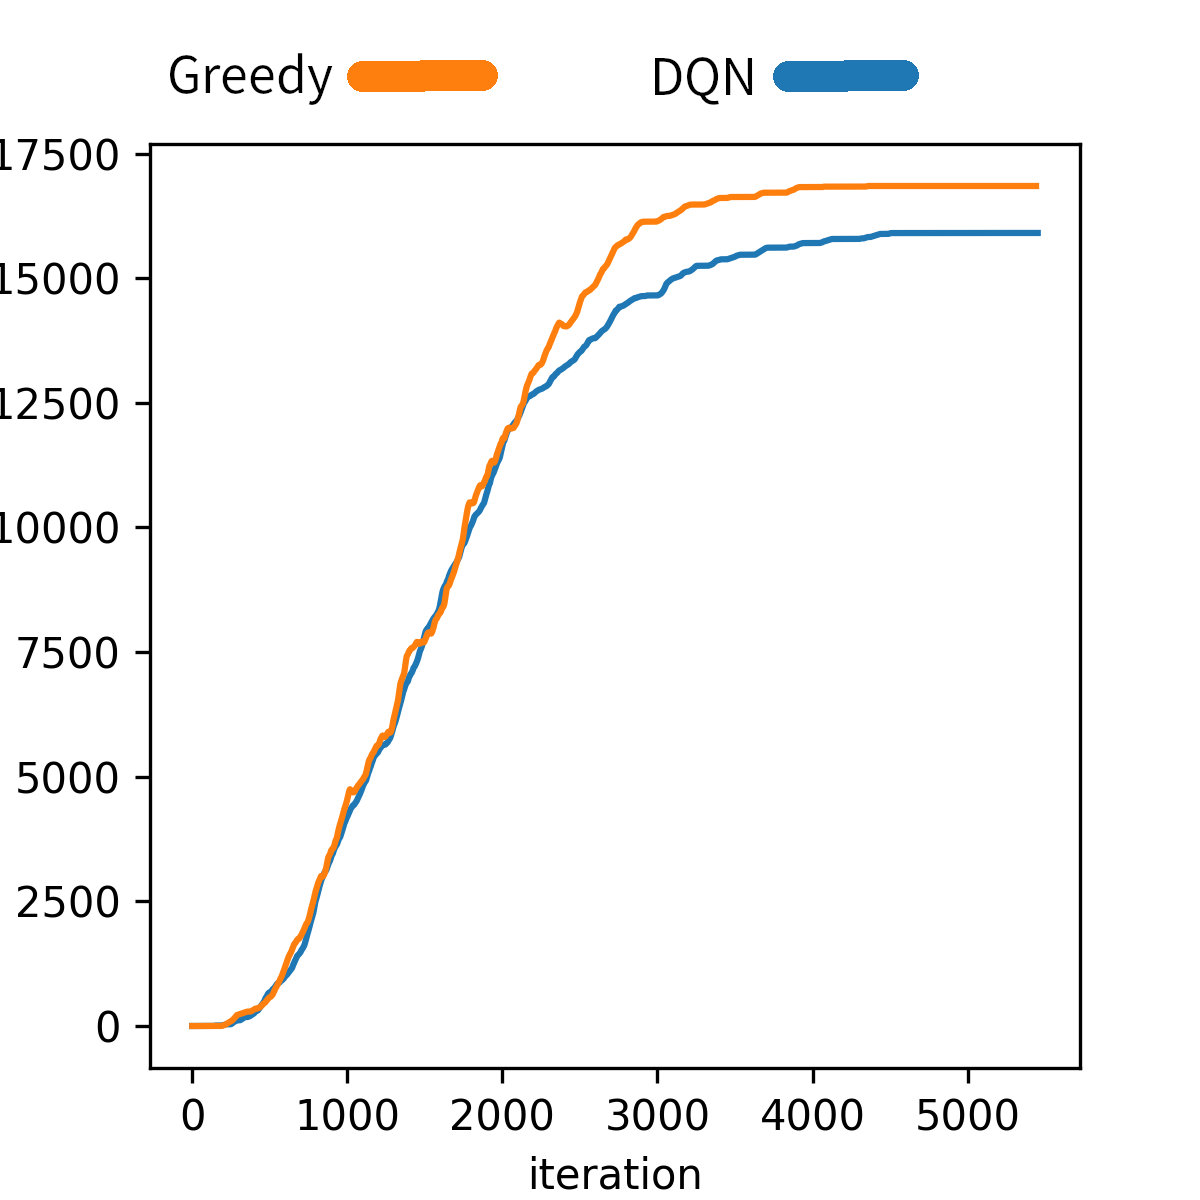
\includegraphics[width=4cm]{waiting_time2.png}}
	\caption{Performance of total waiting time}
	\label{fig:waitingtime}
\end{figure}

Waiting time demonstrates the total cars waiting time of each control policy. 
Slope of Periodic Cycle and Random is much higher than slope of Greedy and Deep Q-Network, meaning that the congestion problems in these two policy are more serious. There is a little difference between Greedy and Deep Q-Network and Greedy has a worse performance. Greedy considers only the current optimal situation, but ignoring some cars which have waited for a long time. Intuitively, because the total number of cars in left turn lane is less than the main road, hence greedy algorithm sacrifices a few cars for the good of all. With gui of simulation, the left turn lane's traffic light is always red during rush hour.

\paragraph{Variance Analysis} During iteration, the variance $\sigma$ is in Figure 4. It's clear that DQN method achieves quite excellent results, compared with other methods.

\begin{figure}[h]
	\centering
	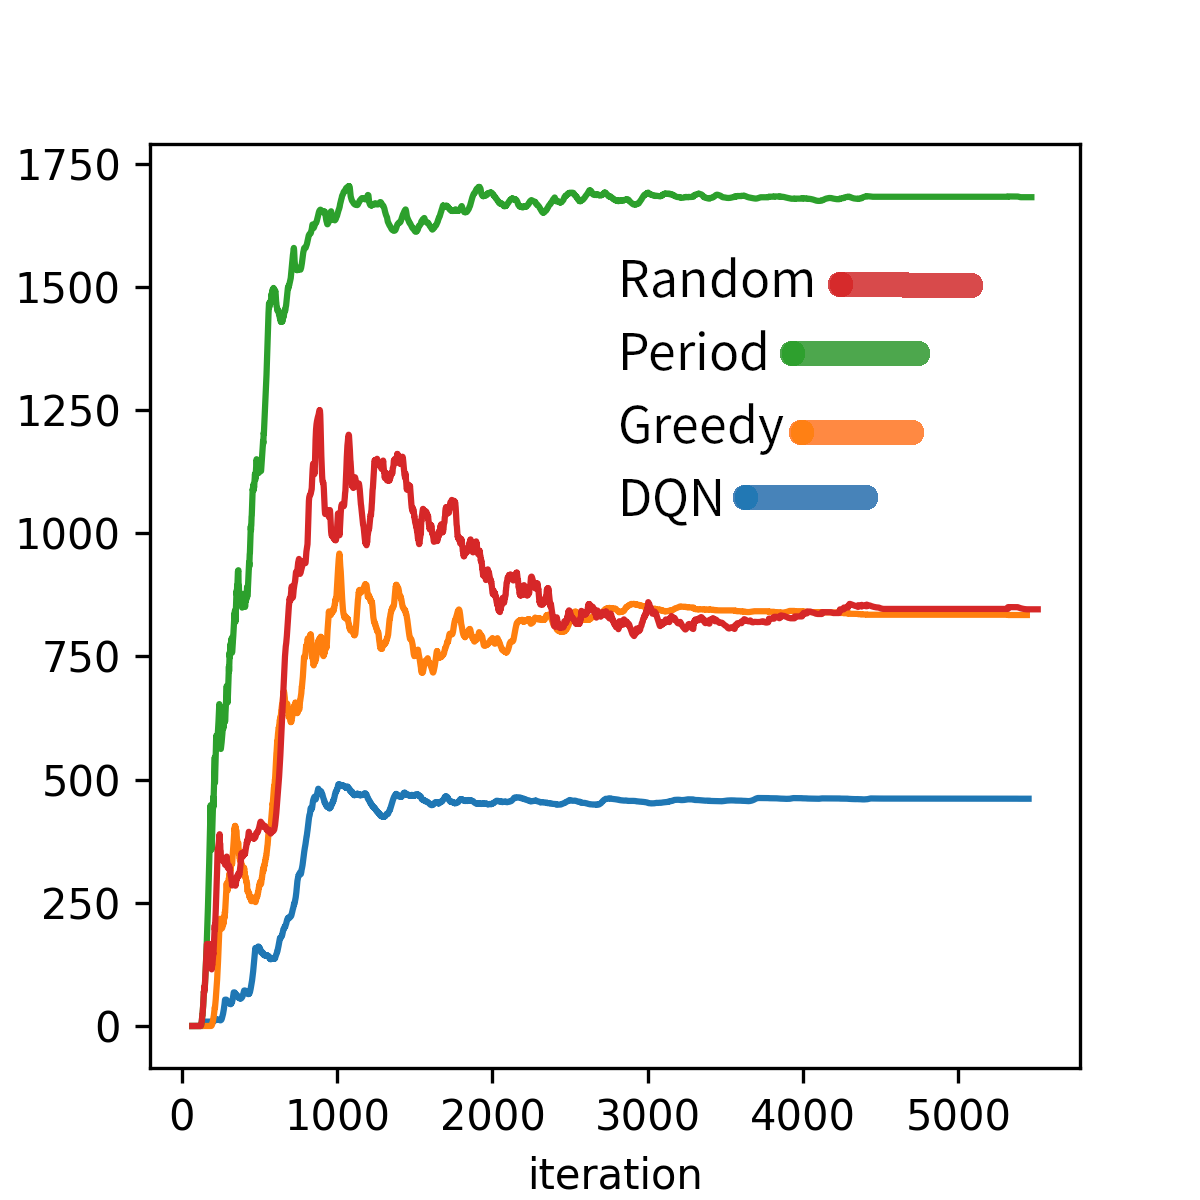
\includegraphics[width=0.75\linewidth]{variance.png}
	\caption{All methods variance}
	\label{fig:variance}
\end{figure}

Variance demonstrates fairness for each vehicle. Above all methods, period method performs worst. It is largely due to the sudden increase of some lanes, but the traffic lights have no reaction to that instant change. Greedy have a lower variance because it can deal with the problem of instant longest vehicle lanes Random performs poorly for every vehicle. And Deep Q-Network performs best, which shows that it can distributes the burden waiting time to all vehicles in a more just way. With gui of simulation, we can clearly find that both greedy and random are hard to properly handle rush hour. Especially greedy algorithm will ignore the left turn lane during rush hour due to there are fewer cars.

\section{6\ \ \ Conclusion}
\hspace*{1em}We have studied the potential of Q-learning, Q-learning with epsilon-greedy, and deep Q-networks (DQN) to optimize real-time traffic signal control policies in intelligent transportation systems. By comparing the performance of these algorithms in a single-intersection scenario, we found that DQN has the best performance in controlling the overall waiting time and variance of waiting time. Naive Q-learning, on the other hand, is impossible to deal with large state spaces and is difficult to converge. While greedy algorithm can achieve good performance, it may sacrifice the waiting time of drivers in the left turn lane (a large variance of waiting time) when there are more cars on the other roads.

In this paper, we focused on the optimal performance achieved in a single-intersection scenario. In reality, it is also important to optimize the signal timings for adjacent Intersection's traffic signals, because the traffic flow at adjacent intersections is correlated. Failing to do so can lead to decisions at one signal that negatively impact traffic operations at another. In the future, we plan to investigate the use of reinforcement learning for more realistic and wide-scale scenarios of traffic lights control. Additionally, different vehicle types (e.g. bus), different speeds of vehivles, pedestrains, security problem (countdown before the light change) and so on, all of these factors are needed to be taken into consideraton when facing a complex reality problem.

\section{Appendix}
\hspace*{1em}As required, at the end of our report, we will list all the external resources (e.g., code, library, tools) that we use and explain how/why we use them.
\paragraph{SUMO} SUMO, Simulation of Urban Mobility, is what we use to simulate urban transportation. It provide the Graphical User Interface (GUI) and Application Programming Interface (API). SUMO provide a python library "traci" as the API. It plays the role of "environment" in reinforcement problem.
\paragraph{PyTorch} As mentioned in section 1.1. PyTorch is one of the most popular deep learning frameworks. It is simple, efficient and fast. To keep our project relevant to the course, PyTorch was used only to help us implement a Multi-Layer Perceptron (MLP) and assist in training the model.
\paragraph{Numpy} NumPy, Numerical Python, is an open source extension of Python for numerical computation. It provides a large number of mathematical function libraries for array operations. We use this library for some common function "argmax" function.
\paragraph{tqdm} "tqdm" module is a python library for progress bar. Without the progress bar, although the code can run normally, but can not provide real-time feedback, blind waiting will cause anxiety, we use "tqdm" to keep us happy.
\end{document}
